
Section~\ref{sec:multipoint-control-plane} describes the procedure
for configuring a multipoint VLAN, and Section~\ref{sec:multipoint-data-plane}
describes a data-plane experiment executed to verify successful provisioning
of the multipoint VLAN.

\subsection{Control Plane Setup}
\label{sec:multipoint-control-plane}

A multipoint VLAN can be created by OESS. However, OSCARS, which is the SDN controller
used for inter-domain circuits, does not support multipoint VLANs. Therefore, we designed
a two-step approach for creating inter-domain multipoint VLANs.

In the \emph{first} step, a point-to-point VLAN was created from the FDT host on each campus, through
the university's regional network, to the corresponding AL2S switch interface. On each campus, the VLAN was configured across the DYNES switch via the corresponding OESS controller. Since
the OESS controller on a campus only controls the DYNES (OpenFlow) switch
and not the remaining campus switches, a campus network administrator was contacted
and asked to provision the VLAN across the remaining campus switches. Since typically
these deployed campus switches are not OpenFlow capable, administrators
either login to each switch to configure VLANs, or use network management tools if available. Similarly, administrators at regional networks were contacted to provision the VLAN through
their switches.

As an example, Fig.~\ref{fig:UVA-VLAN336} shows VLAN 336 that
was provisioned across the UVA DYNES switch using OESS, through the campus switches by
a UVA campus network administrator, and across the MARIA regional network by a MARIA
administrator. The provisioned VLAN 336 terminates on port et-3/0/0.0 of the Internet2 AL2S Ashburn switch as shown in Fig.~\ref{fig:UVA-VLAN336}.
\begin{figure}[htb!]
\centering
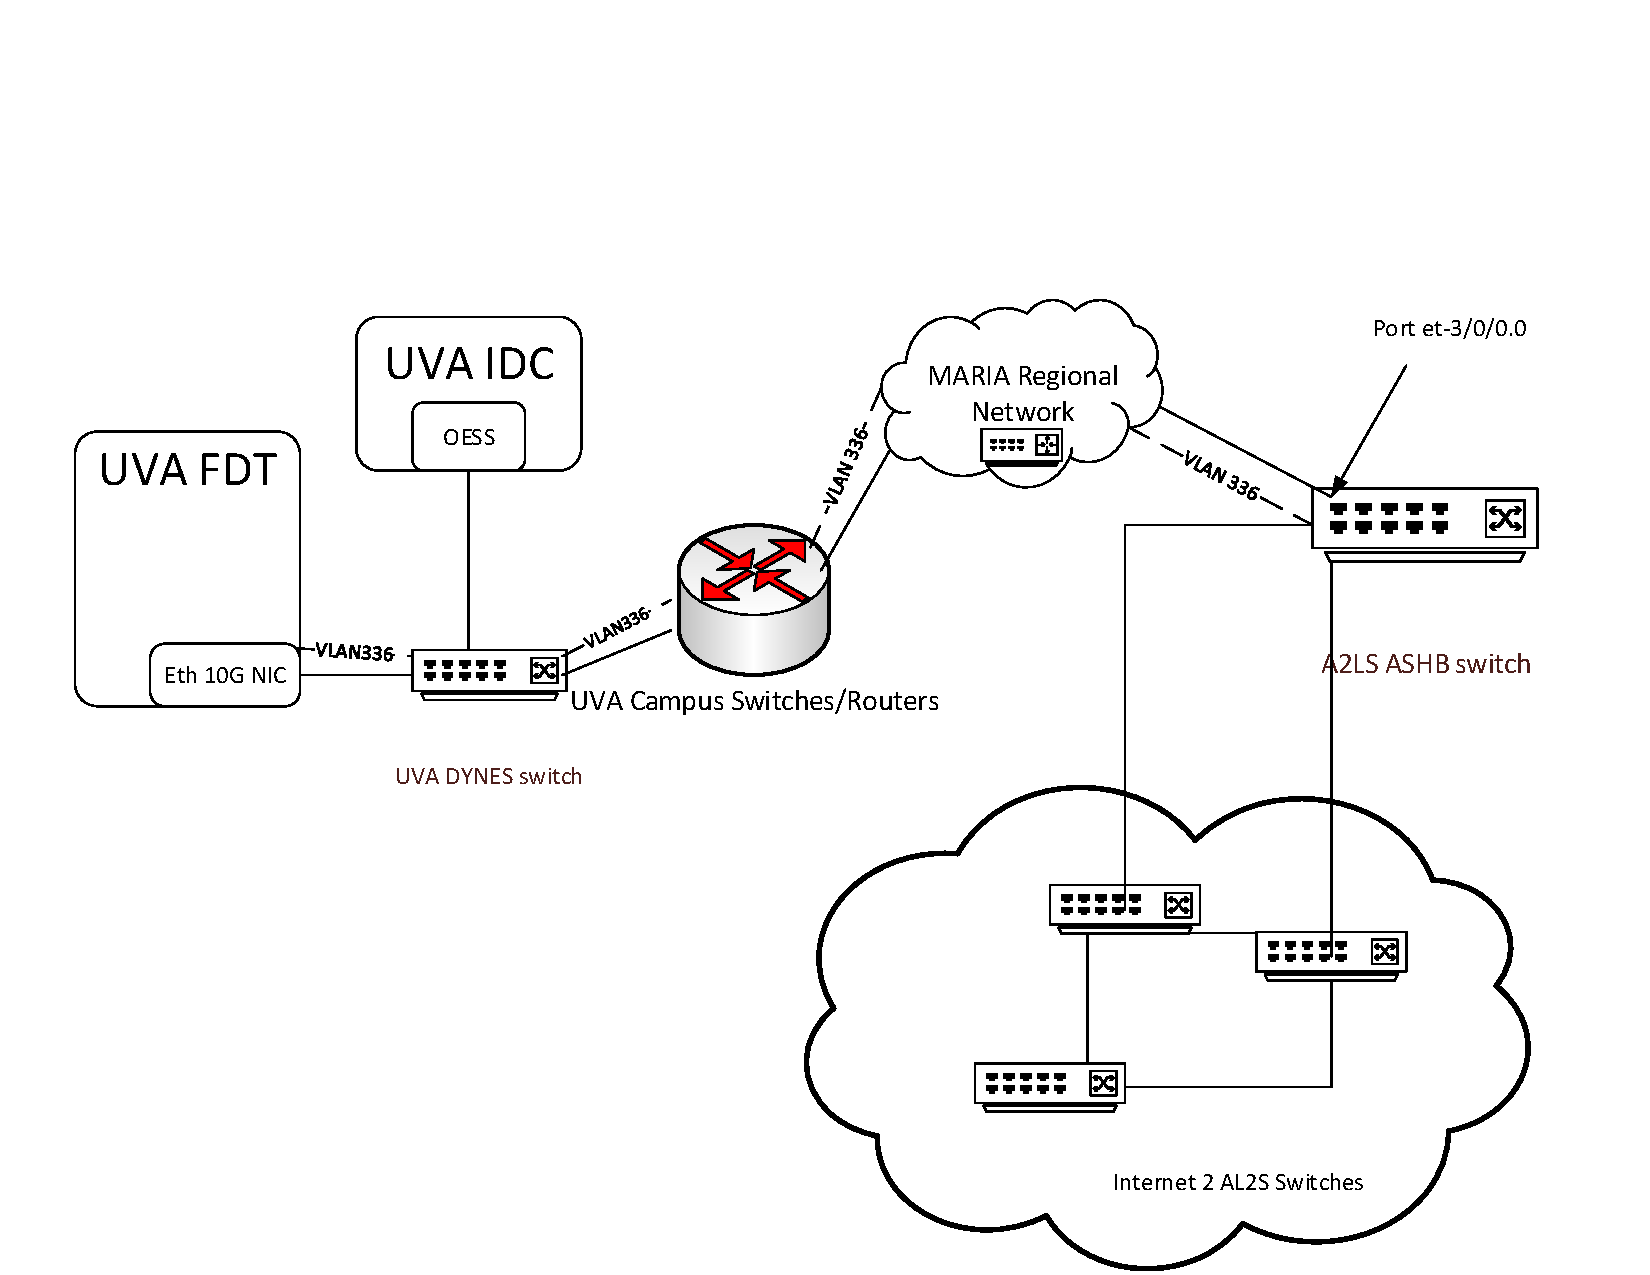
\includegraphics[width=0.8\textwidth]{figures/UVA-ASHB.pdf}
\caption{UVA DYNES - UVA campus – MARIA- ASHB}
\label{fig:UVA-VLAN336}
\end{figure}

One such provisioned VLAN was established from each campus FDT to a specific
port of an Internet2 AL2S switch. Since campus network and regional network
administrators assign VLANs for many purposes, it is unlikely to obtain the
same VLAN ID for all campus/regional networks. Already, there is some constraint
in that each campus administrator has to collaborate with the corresponding
regional network administrator to select a common range of VLANs that is still available
for allocation. One or more VLAN IDs from this range is then used in the
above-described manual provisioning process. Therefore,
the VLAN ID selected by each campus/regional network on the multipoint VLAN
could be different. This was the case for the three-point VLAN illustrated
in Fig.~\ref{fig:wanmulticast}. The VLAN ID used for the UVA-MARIA path was 336,
the VLAN ID used for the MAX path (MAX is a regional network, and hence there
is no corresponding university campus) was 1830, and the VLAN ID on the IU-Indiana
GigaPoP path was 2399.
\begin{figure}[htb!]
\centering
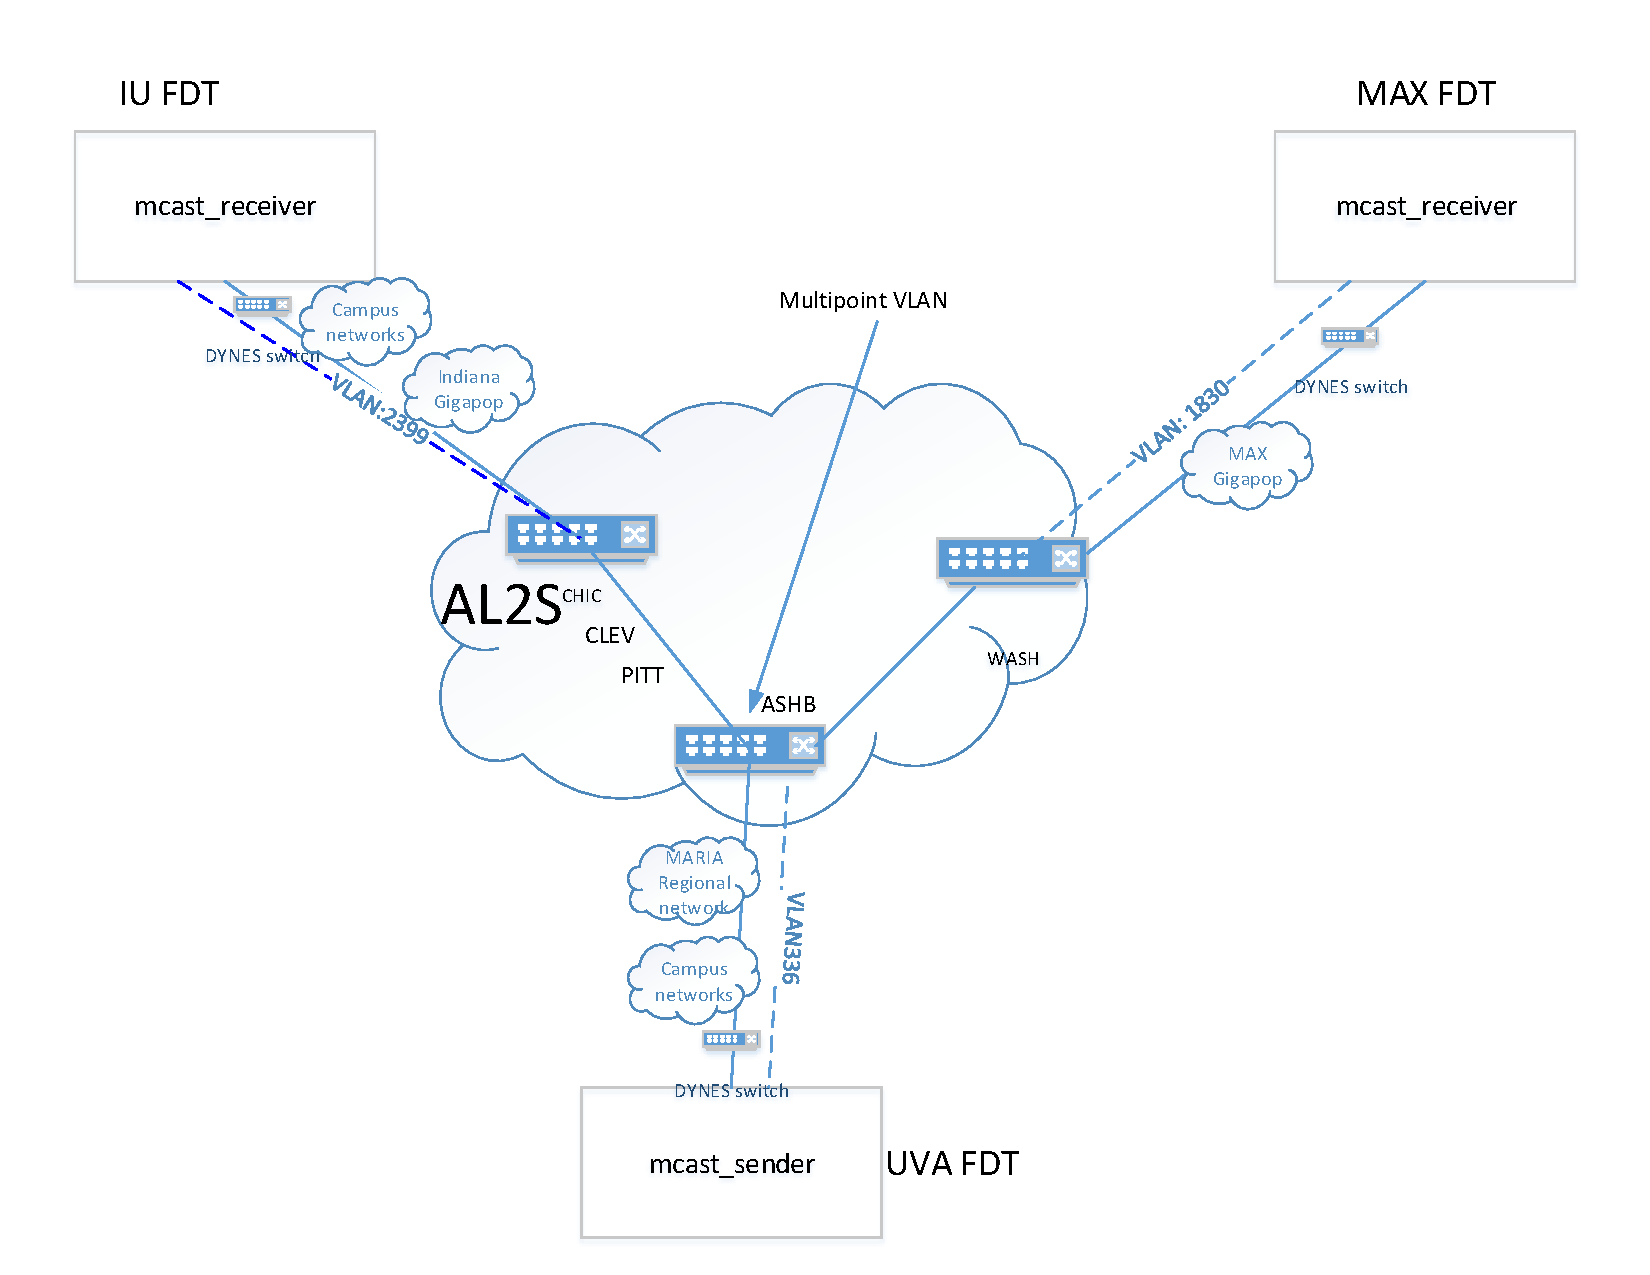
\includegraphics[width=0.8\textwidth]{figures/AL2S-mcast.pdf}
\caption{AL2S inter-domain multipoint circuit experiment}
\label{fig:wanmulticast}
\end{figure}

The second step consists of provisioning the intra-domain multipoint VLAN
across the Internet2 AL2S network as illustrated in Fig.~\ref{fig:oessal2s}.
Three endpoints are interconnected via this multipoint VLAN:
(i) MARIA's connection to interface \texttt{et-3/0/0.0} of Internet2 AL2S switch \texttt{sdn-sw.ashb.net.internet2.edu} (Ashburn, VA switch) with VLAN ID 336,
(ii) and MAX Gigapop's connection to interface \texttt{eth3/2} of Internet2 AL2S switch \texttt{sdn-sw.wash.net.internet2.edu} (McLean, VA switch) with VLAN ID 1830, (iii) and Indiana Gigapop's connection to interface \texttt{eth1/2} of Internet2 AL2S switch \texttt{sdn-sw.chic.net.internet2.edu} (Chicago, IL switch) with VLAN ID 2399.
\begin{figure}[htb!]
\centering
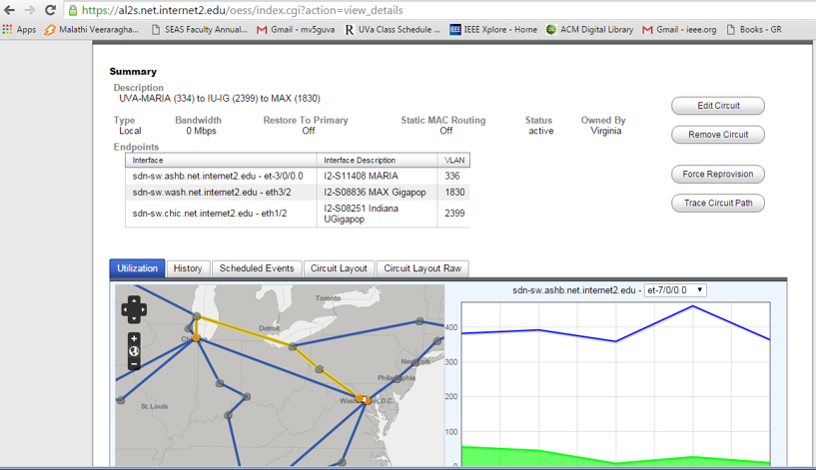
\includegraphics[width=0.8\textwidth]{figures/oess-AL2S.png}
\caption{AL2S OESS: Endpoints and VLAN selection}
\label{fig:oessal2s}
\end{figure}

The OpenFlow switch at the Internet2 AL2S Ashburn location is performing a complex function. 
For each VLAN-ID-336-tagged packet received on its port \texttt{et-3/0/0.0}, the Ashburn
switch makes two copies, and rewrites the VLAN ID in one copy to 2399 and to 1830 in the second copy.
The switch then sends the VLAN-ID-1830-tagged packet to port \texttt{et-1/3/0}, and sends VLAN-ID-2399-tagged packet to port \texttt{et-7/0/0}.
Similarly, each packet received with VLAN ID 2399 on port \texttt{eth1/2} in Internet2 AL2S Chicago switch is duplicated, and one copy is sent to Ashburn switch
with VLAN ID rewritten to 336, and the second copy is sent to Washington switch with VLAN ID rewritten to 1830,
and each packet received with VLAN ID 1830 on port \texttt{eth3/2} in AL2S Washington switch is duplicated with VLAN ID rewritten, and sent one copy with VLAN ID 336 to Ashburn and second copy with VLAN ID 2399 to Chicago switch.


As the Internet2 AL2S switches support only OpenFlow 1.0, it was surprising that these switches
support this complex copying and rewriting functionality. Nevertheless, this feature was
most useful for our multipoint VLAN provisioning.

\subsection{Data-Plane Experiments}
\label{sec:multipoint-data-plane}

The software used in these data-plane experiments consists of: (i) a multicast application for sending and receiving multicast traffic, (ii) Linux utility \texttt{vconfig} to configure VLAN IDs (tags) on host NICs,  (iii) Linux \texttt{ifconfig} to configure IP address and subnet mask for the configured VLAN, (iv) Linux utility \texttt{ping} to test the reachability on a VLAN, and (v) Linux utility \texttt{tcpdump} to capture multicast packets.

First, we describe a local (single-domain) multipoint experiment. Next, we present the results of
an inter-domain multipoint VLAN test.

\paragraph{Single-domain multipoint experiment}
\begin{figure}[htb!]
\centering
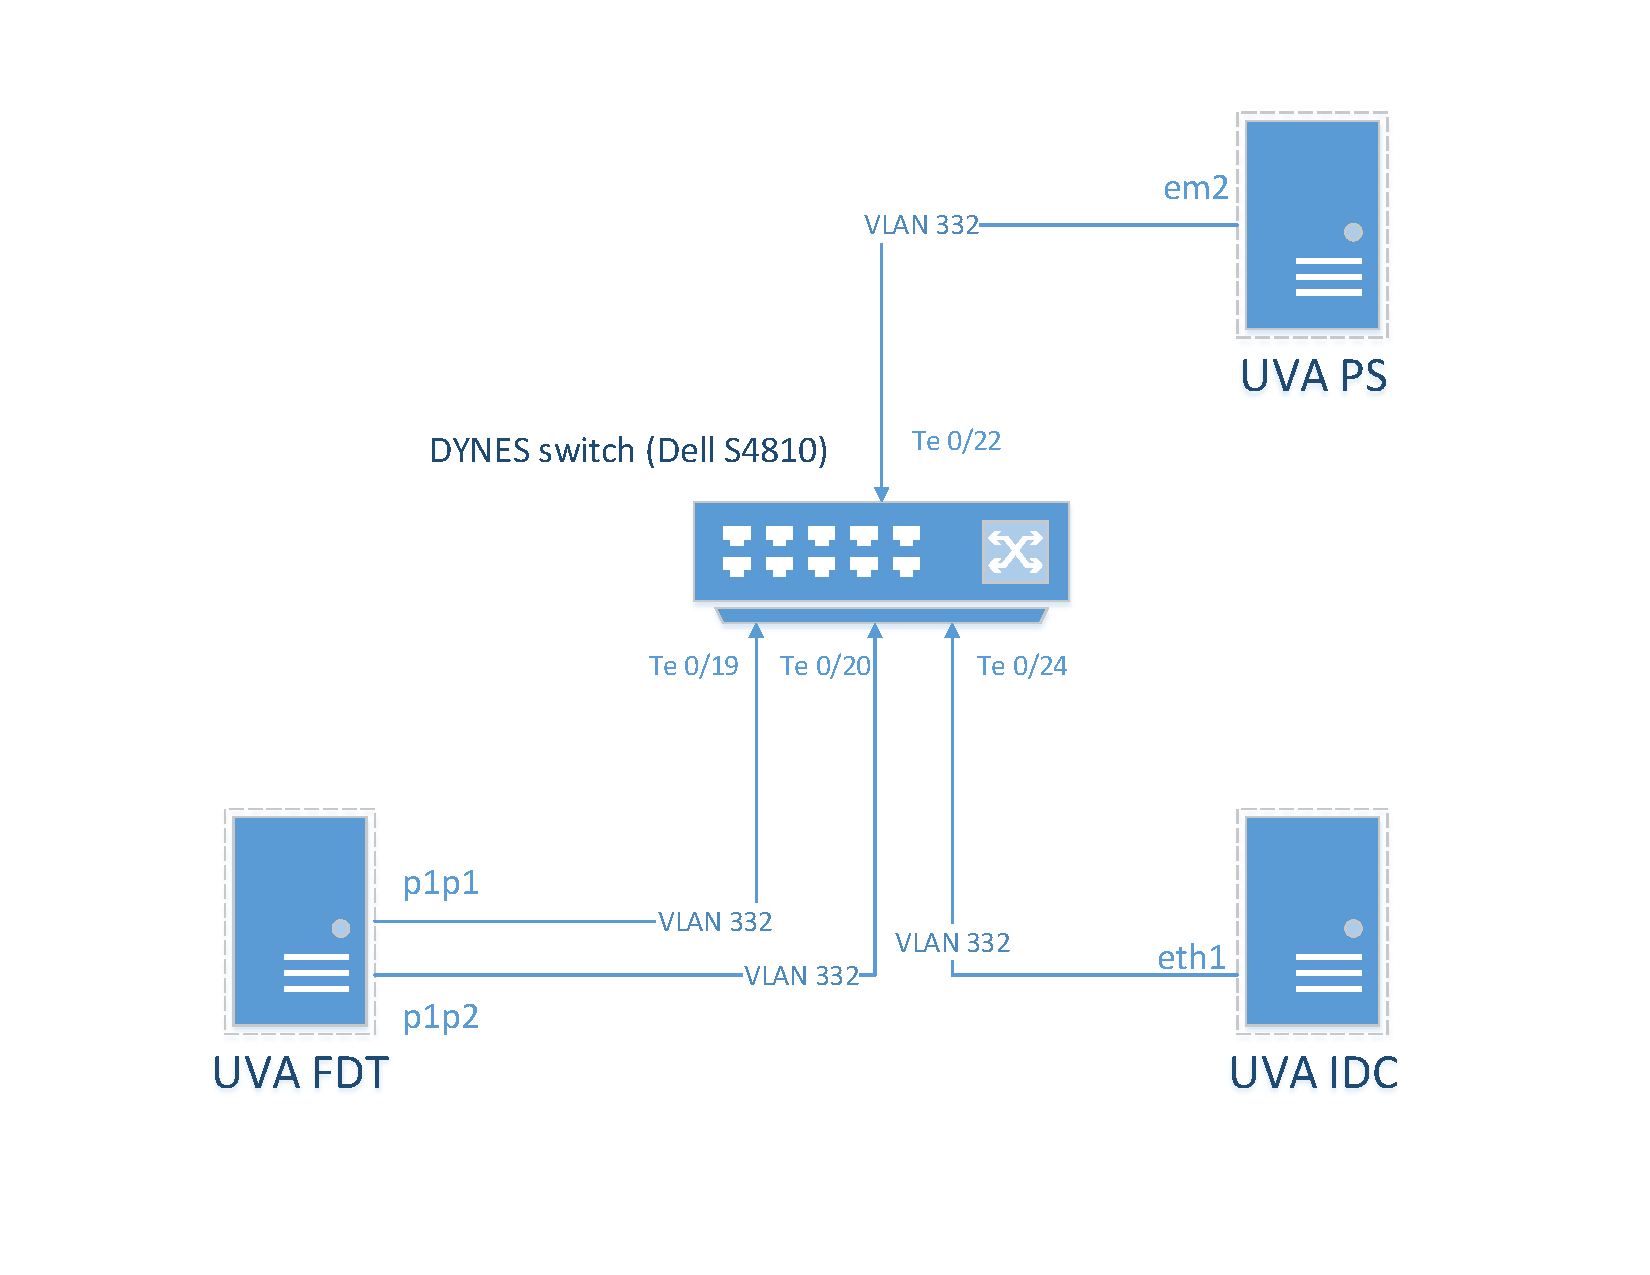
\includegraphics[width=0.8\textwidth]{figures/single-domain.pdf}
\caption{A local multipoint VLAN configuration through the UVA
DYNES switch connecting FDT, PS and IDC host}
\label{fig:single-domain}
\end{figure}

The multicast application was tested across an intra-domain multipoint VLAN. Fig.~\ref{fig:single-domain} shows the multipoint
VLAN configuration through the UVA DYNES switch connecting FDT, PS and IDC hosts. The same VLAN ID 332
is used on all three interfaces. The UVA DYNES switch, which is a Dell S4810 OpenFlow 1.0 switch, does not support multicasting
with VLAN ID rewrite, which implies that the same VLAN ID needs to be used on all interfaces.
This VLAN was created using OESS.
Fig.~\ref{fig:flowtable} shows one of the three OpenFlow flow-table entries created in the UVA DYNES switch by the OESS. When the switch receives a VLAN-332-tagged packet on port Te 0/19, the switch looks up the OpenFlow
table and finds a match for this packet with the entry shown in Fig.~\ref{fig:flowtable}. The switch then
replicates the packet, and sends one packet to each of three ports: Te 0/20, Te 0/22, Te 0/24. All three packets will be tagged with the same VLAN ID 332, as per the specifications of the OpenFlow flow-table entry
shown in Fig.~\ref{fig:flowtable}.

After the OpenFlow multipoint VLAN was set up via OESS, we configured VLANs at each of the three hosts
 using the process described in Section~\ref{sec:multidomain-SDN-FDT-access}. Private IP addresses on the same subnet were
 assigned to the VLANs at these hosts. Next, we used the \texttt{ping} utility to verify connectivity
 via this multipoint VLAN.

\begin{figure}[htb!]
\centering
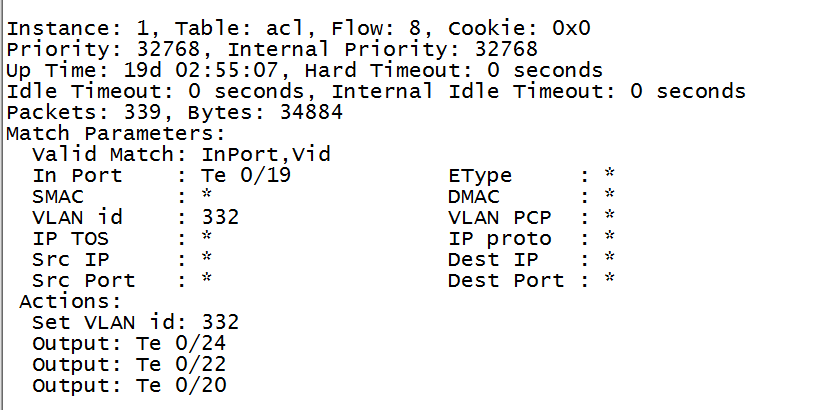
\includegraphics[width=0.8\textwidth]{figures/flow-table.png}
\caption{OpenFlow flow-table entry in the UVA DYNES switch}
\label{fig:flowtable}
\end{figure}

Second, a Linux multicast application was run to test the multipoint VLAN. The application
consists of a multicast sender (\texttt{mcast\_sender}) and a multicast receiver (\texttt{mcast\_receiver}).
We executed the \texttt{mcast\_sender} program on the UVA FDT, and the \texttt{mcast\_receiver} program
on the other two UVA DYNES hosts (IDC and PS).
As Fig.~\ref{fig:localmulticast} shows the unicast IP addresses of the VLAN at each host needs
to be specified as the first argument of both \texttt{mcast\_sender} and \texttt{mcast\_receiver}. These
IP addresses are 10.30.32.20 for the FDT NIC VLAN 332, 10.30.32.30 for the IDC NIC VLAN 332, and 
10.30.32.40 for the PS NIC VLAN 332. The specified unicast IP address is associated with the UDP socket
at each host that was opened with the \texttt{mcast\_sender} and \texttt{mcast\_receiver} using the multicast IP address 233.0.225.123 (which is the second argument). The last argument of both programs is the UDP port number 8888. 
Therefore, within the code, the second and third arguments are used to create a UDP socket. Then using
the Linux \texttt{setsockopt} system call, the unicast IP address provided as the first argument is associated
with the UDP socket. All datagrams passed to this UDP socket by the application are then sent to the interface
associated with the unicast IP address. The reason for associating a unicast IP address with the UDP socket that was created
with the multicast IP address is to avoid having to set an IP routing table entry corresponding
to the multicast IP address at the sending host. For example, if the sender has two NICs,
there could be an IP routing table entry for
the IP multicast address range to send packets to one of the two NICs, while the multipoint VLAN
could be configured to use the second NIC. In this case, either a new IP routing table entry is required
to direct packets addressed to the particular IP multicast address to the second NIC,
or the \texttt{setsockopt} function should be called by the application opening the multicast UDP socket
to associate the unicast IP address of the interface to which the multicast packets should be sent with that socket. In this case \texttt{mcast\_sender} and  \texttt{mcast\_receiver} perform the latter function. Since the unicast IP address provided is that of VLAN 332 in all
three hosts, all multicast packets will have a UDP header, an IP header with destination IP address set
to 233.0.225.123, an Ethernet header and an IEEE 802.1Q header with the VLAN ID set to 332. 
\begin{figure}[htb!]
\centering
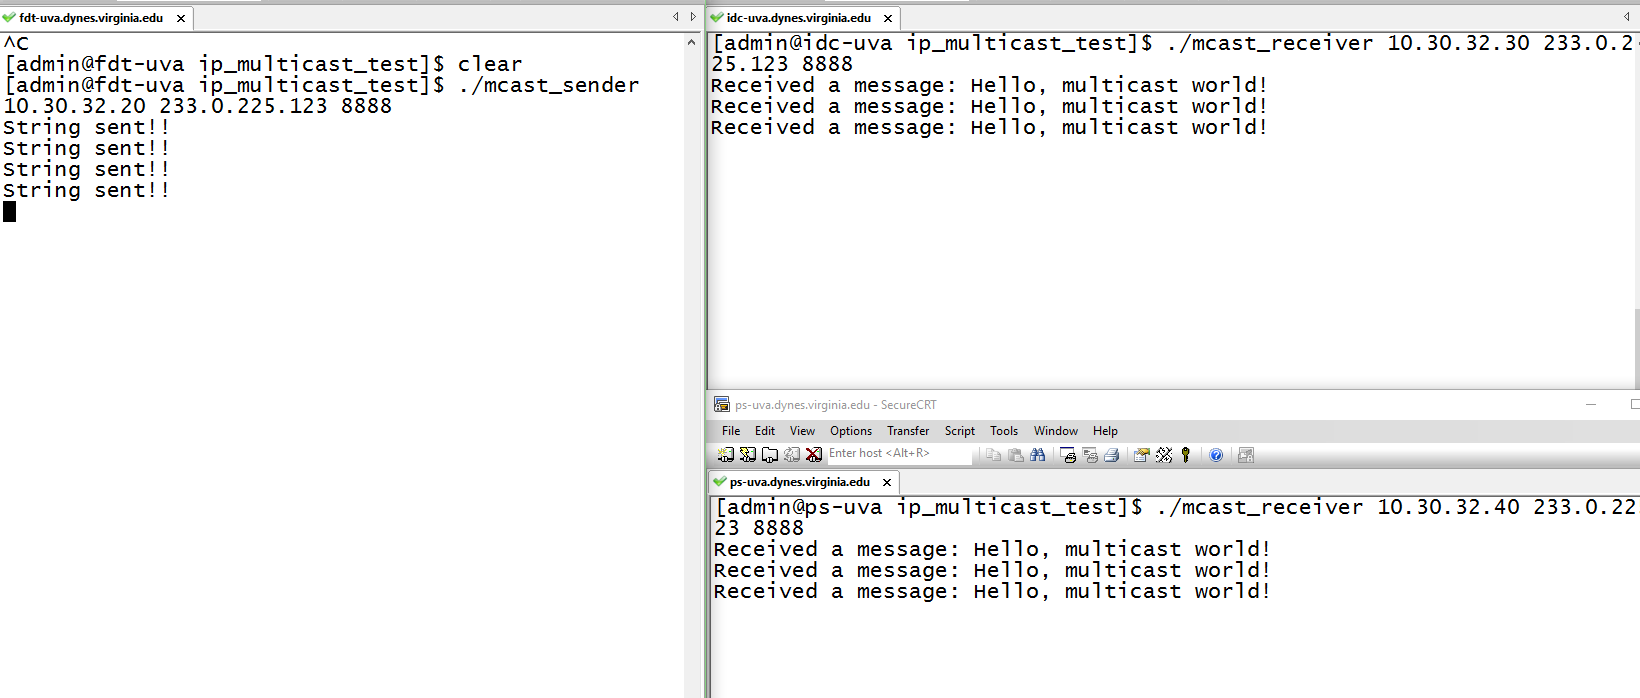
\includegraphics[width=0.8\textwidth]{figures/local-multicast.png}
\caption{Multicast application sending traffic from UVA FDT to UVA PS and UVA IDC hosts across a local multipoint VLAN}
\label{fig:localmulticast}
\end{figure}

The 233.0.225.123 IP address belongs to the 
GLOP range. The GLOP address IP range, 233.0.0.0/8, was assigned as an experimental address space for IP multicast service providers and networking researchers. The convention is to use the 16-bit autonomous system number (ASN)
in the second and third bytes. Since UVA's ASN is 225, the second and third bytes of our select multicast IP address 233.0.225.123 are 0 and 225, respectively.  

When the UVA FDT \texttt{mcast\_sender} program sent the message ``Hello, multicast world!'', the
\texttt{mcast\_receiver}  program running on the IDC and PS hosts received the message. However, when we changed the VLAN tags of these 3 interfaces to different values in local OESS, the related flow entries were not set in the flow table of UVA DYNES switch since multipoint VLAN tag translation feature was not supported in Dell  switch.
\begin{figure}[htb!]
\centering
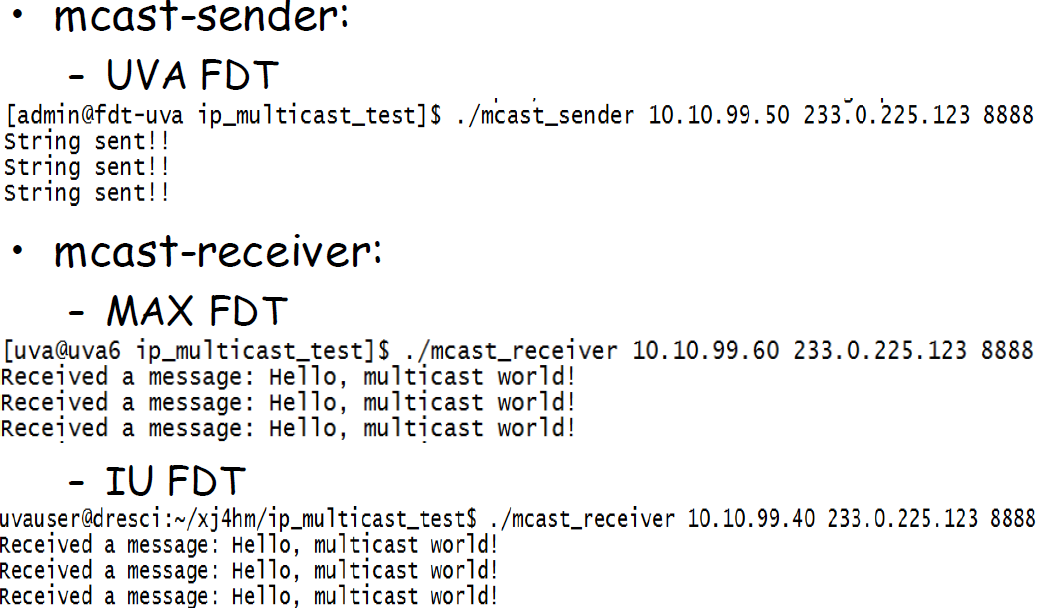
\includegraphics[width=0.8\textwidth]{figures/AL2Smulticast.png}
\caption{Multicast application sending traffic from UVA FDT to MAX FDT and IU FDT across an inter-domain multipoint VLAN}
\label{fig:widemulticast}
\end{figure}

\paragraph{Inter-domain multipoint experiment}
The control-plane actions for provisioning an inter-domain multipoint VLAN  were described in Section~\ref{sec:multipoint-control-plane}. These actions were executed to create a multipoint VLAN
between UVA FDT, MAX FDT and IU FDT. Specifically, this multipoint VLAN, with three different VLAN IDs, was illustrated
in Fig.~\ref{fig:oessal2s}.

The multicast application described above was then executed across this inter-domain multipoint VLAN. Fig.~\ref{fig:widemulticast} shows that the \texttt{mcast\_sender} program was executed at the UVA FDT,
and the \texttt{mcast\_receiver} program was executed at the MAX FDT and IU FDT. The ``Hello, multicast world!''
message sent by the \texttt{mcast\_sender} program running on the UVA FDT was successfully received by the 
\texttt{mcast\_receiver} processes at the MAX FDT and IU FDT.

\begin{figure}[htb!]
\centering
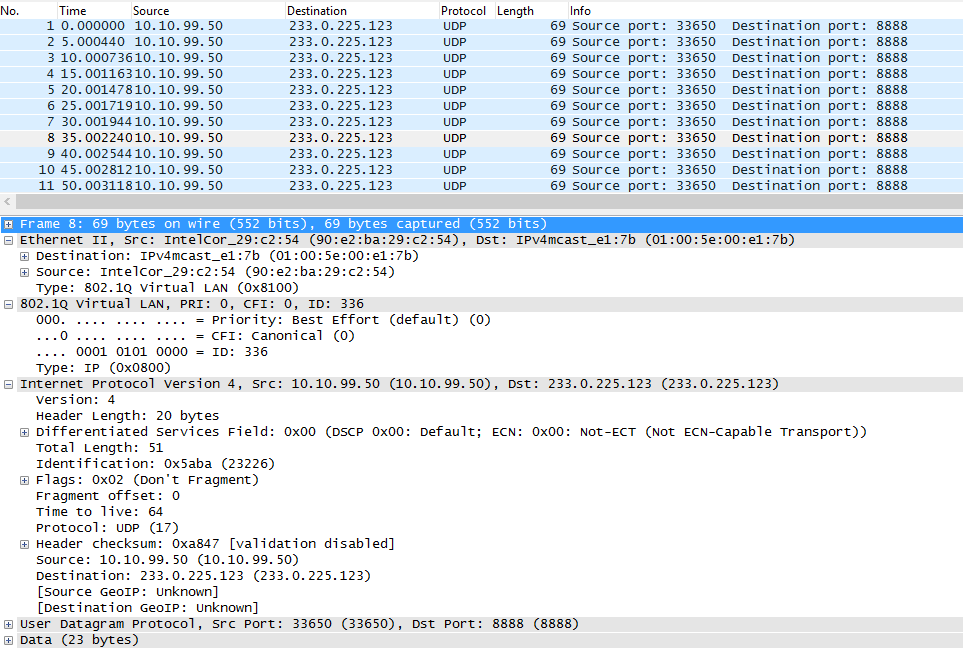
\includegraphics[width=0.8\textwidth]{figures/pcap.png}
\caption{Wireshark display of a pcap file}
\label{fig:multicast-pcap}
\end{figure}
To verify that packets were being multicast across the inter-domain multipoint VLAN, packets were captured with the \texttt{tcpdump} utility at the UVA FDT. Fig.~\ref{fig:multicast-pcap} shows some of the header fields, such as Source and Destination IP addresses, for the multicast packets. The source IP address is 10.10.99.50, which is the IP address assigned to VLAN 336 on the UVA FDT NIC, and the destination IP address is the GLOP IP address 233.0.225.123.
The destination MAC address of the Ethernet header, as seen in the lower window of Fig.~\ref{fig:multicast-pcap} is 01:00:5e:00:e1:7b, which is explained next.

Fig.~\ref{fig:mapping} shows the mapping solution used for multicast IP addresses. This solution is different
from the mapping procedure used for unicast IP addresses. To find the MAC address corresponding
to a unicast IP address, the Address Resolution Protocol (ARP) is used in which a request carrying the unicast
IP address being mapped is broadcast to all interfaces, and the interface whose IP address matches the address in the
request responds with its MAC address. However, for a multicast IP address, a single Ethernet MAC address
is required so that a single Ethernet frame, carrying the IP multicast packet, can be received by multiple receivers.
All multicast receiver NICs need to be configured with a multicast MAC address so that all these receivers will accept Ethernet frames whose destination MAC address matches the configured multicast MAC address. Without such a
multicast MAC address configuration, each  NIC will only accept Ethernet frames whose destination MAC address equals its own unicast MAC address and frames whose destination MAC address is 0xFF:FF:FF:FF:FF:FF (broadcast address). Therefore, when the \texttt{mcast\_sender} or \texttt{mcast\_receiver} program creates the \texttt{ipm} (IP-multicast) socket, the code calls the Ethernet driver to configure the NIC with another MAC address, 01:00:5e:00:e1:7b, so that the NIC accept accept frames with this destination MAC address. The Wireshark analysis of the captured packets verifies that this procedure
is being executed.
\begin{figure}[htb!]
\centering
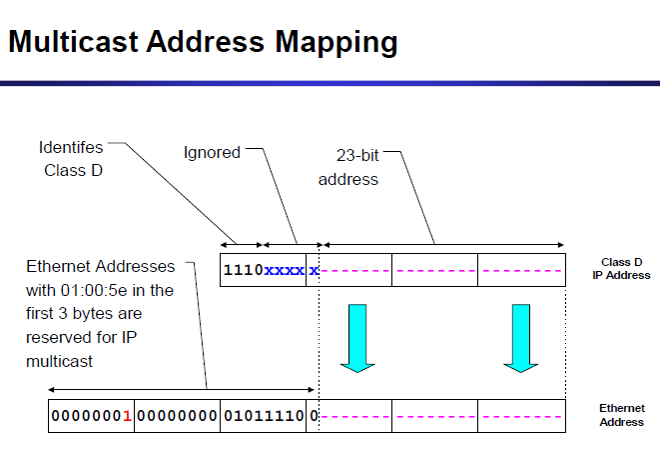
\includegraphics[width=0.8\textwidth]{figures/mapping.png}
\caption{Multicast IP address to multicast MAC address mapping}
\label{fig:mapping}
\end{figure}


\paragraph{Key Findings}
The key findings of the experiments are as follows: (i) multipoint VLANs that require VLAN ID translation (rewrite) is supported by at least some of the Internet2 AL2S switches, which allows for the creation of inter-domain multipoint VLAN. This finding is important for the deployment of LDM7, which was our motivating application to pursue SDN-controlled path-based networking in general, and multipoint VLANs in particular. (ii) Packets with the multicast destination IP address were dropped by firewalls in some campus networks and some regional networks. A systematic method is required for debugging connectivity across multiple domains.

